\documentclass[a4paper]{ctexart}
\usepackage{xeCJK}
\usepackage{setspace}
\usepackage{graphicx,wrapfig}
\usepackage{fontspec,xunicode,xltxtra}
\usepackage{fancyhdr,titlesec,titletoc}
\usepackage[titletoc]{appendix}
\usepackage[top=29mm,bottom=29mm,left=31.8mm,right=31.8mm]{geometry}
\usepackage{enumerate,enumitem}
\usepackage{caption}
\usepackage{amsmath,amssymb,bm,array}
\usepackage{cite}
\usepackage{diagbox}
\usepackage{algorithm,algorithmicx,algpseudocode}
\usepackage{multirow}
\usepackage[super]{gbt7714}
\setmainfont{Times New Roman}
%\setCJKmainfont{SimSun}
\setCJKfamilyfont{heiti}{SimHei}
\renewcommand{\heiti}{\CJKfamily{heiti}\fontspec{Times New Roman}}

\newcommand{\mycaptionfont}{\heiti\zihao{5}}
\captionsetup[figure]{name={\mycaptionfont 图},labelsep=period}
\captionsetup[table]{name={\mycaptionfont 表},labelsep=period}
\floatname{algorithm}{\mycaptionfont 算法}
\captionsetup[algorithm]{labelsep=period}
\renewcommand{\captionfont}{\mycaptionfont}
\renewcommand{\captionlabelfont}{\mycaptionfont}

\ctexset {
	section = {
		number = \arabic{section},
		format = \zihao{4}\bfseries,
	},
	subsection = {
		number = \arabic{section}.\arabic{subsection},
		format = \zihao{-4}\bfseries,
	},
	subsubsection = {
		number = \arabic{section}.\arabic{subsection}.\arabic{subsubsection},
		format = \zihao{-4}\bfseries,
	}
}
\setlist[enumerate]{itemindent=2em,listparindent=2em,leftmargin=0em,label=\arabic*、}

\setlength\parskip{.5\baselineskip}
\fancypagestyle{plain}{\pagestyle{fancy}}%改变章节首页页眉
\pagestyle{fancy}
\lhead{\kaishu~《人工智能》课程作业~}
\rhead{\kaishu~201857~尹达恒}
\cfoot{\thepage}

\renewcommand{\abstractname}{摘要}
\renewenvironment{abstract}{
	\quotation
	\begin{spacing}{1.2}
		\par\zihao{5}{\bfseries \abstractname:}
	}{\end{spacing}\vskip 2.5ex}

\begin{document}
\begin{center}
	{\zihao{-3}\textbf{面向实时交互式视频通信客户端侧流量调节的智能Agent设计和关键技术}}

	{\zihao{-4}尹达恒}\\[-1mm]

	{\zihao{5}(东南大学,江苏\quad 南京)}
\end{center}
\begin{abstract}
	本文面向实时交互式视频通信领域,提出了一种基于强化学习和联邦学习的客户端侧流量调节的智能Agent设计方案,并针对关键问题和相关研究现状阐述了构建Agent所需的技术,最后对整体实现方案进行了可行性分析。

	本文所设计的系统解决了实时交互式视频通信领域的几个重要问题,功能完善,为大规模实时交互式视频通信应用的构建提供了有力支持,具有较强的实用价值。

	\textbf{主题词:} 视频流,策略搜索,流量调节,联邦学习,强化学习
\end{abstract}
\renewcommand{\baselinestretch}{1.3}
\zihao{5}

\section{场景描述}

2020年的新冠肺炎疫情对传统的面对面“接触式”办公模式带来了巨大的冲击,作为“无接触式”办公模式的重要组成部分,视频会议软件得到的空前的发展,实时交互式视频通信应用迅速渗透到各行各业的生产活动中。

根据Cisco发布的年度网际网络报告(Cisco Annual Internet Report)\cite{CiscoAnnualInternetReport},在当今的所有互联网流量中,实时交互式视频流量占据着主导地位。随着LTE-Advanced和5G的发展,新的低延迟应用也在迅速出现,例如实时视频/VR广播、云游戏、手术机器人或车辆的远程操作等。这样的交互式视频应用比视频会议应用在带宽和延迟方面的要求更加苛刻。尽管电信基础设施努力满足需求,但基础设施仅能提供尽力而为的服务,因此,为了适应高度动态的网络条件和不同应用场景多样化的需求,在交互式视频通信客户端一侧的流量调节必不可少。

\begin{enumerate}[label=\arabic*、]
	\item 应用领域:交互式视频通信;
	\item 主要功能:在客户端一侧,根据网络环境实时地调节流量策略。
\end{enumerate}

\section{智能化任务}

在上述在交互式视频通信客户端一侧调节流量的应用场景中,人工智能算法需要处理的智能化任务可以概括为:

\begin{itemize}
	\item 输入:算法要能够及时地获取客户端一侧当前网络情况;
	\item 输出:算法要需要根据获取到的网络情况调节视频编码的比特率;
	\item 优化目标:视频编码的比特率应该调节到恰好使网路不发生拥塞。
\end{itemize}

\section{任务环境分析}\label{sec:任务环境分析}

智能Agent的任务环境图\ref{figure:env}所示。本节将从Agent的输入输出和优化目标出发对Agent的任务环境进行分析。

\begin{figure}[htbp]
	\centering
	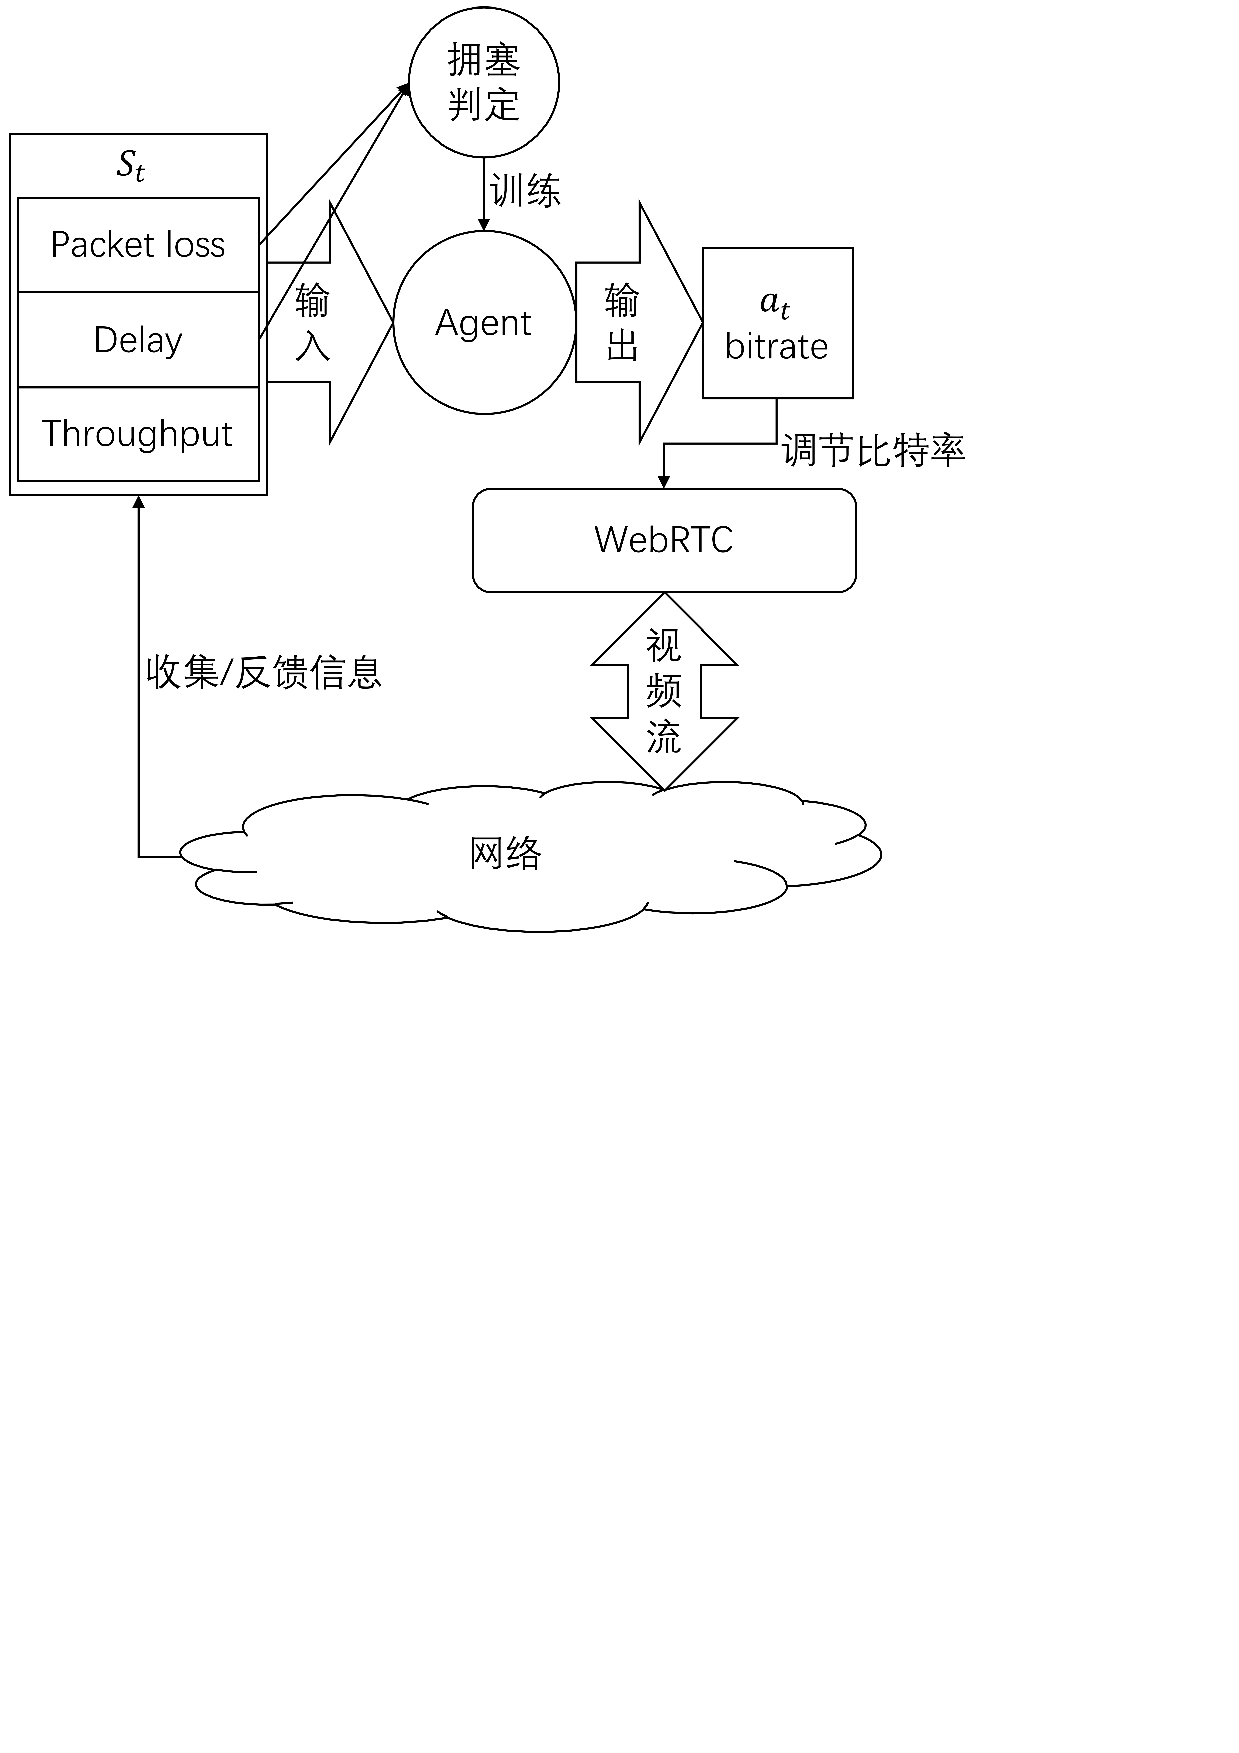
\includegraphics[width=0.9\textwidth, keepaspectratio]{figure/env.pdf}\\
	\caption{智能Agent的任务环境}\label{figure:env}
\end{figure}

\subsection{Agent输入分析}

网络情况所涵盖的变量很多,但大部分变量都记录在路由器、交换机等运营商侧的设备中。显然,实际情况下,运营商不可能在机房中大面积部署高能耗的人工智能应用,也不大可能将通信设备的状况信息开放给用户获取。因此,在客户端侧,Agent所能获取到的信息是比较有限的。根据目前交互式视频通信常用的传输/应用层协议 —— WebRTC的内容,Agent可以通过协议中周期性的RTCP ACK消息收集到每个数据包的发送情况,继而计算出如下的网络状况信息:

\begin{enumerate}[label=\arabic*、]
	\item 丢包率(Packet loss)$l_t$:根据TCP协议中的超时重传规则,在TCP协议中对正常发送的包和重传包进行计数,即获取一定时间内的丢包率信息;
	\item 延迟(Delay)$d_t$:根据TCP协议的ACK机制,对包发送完成和收到确认ACK的时间间隔进行计数,即可获得发送过程的延迟信息;
	\item 吞吐量(Throughput)$t_t$:根据TCP协议中的发送机制,统计一定时间内的发送窗口和接收窗口大小,即可获得系统的吞吐量信息。
\end{enumerate}

令$S_t=(l_t, d_t, t_t)$表示第$t$个计时区间内Agent输入的网络状况信息。

\subsection{Agent输出分析}\label{sec:Agent输出分析}

由于视频流需要连续发送的特点,在设计Agent时可以不必考虑包发送的时刻问题,而只用考虑一段时间内发送包的数据总量,即视频流的比特率。目前视频流应用常用的WebRTC框架即具有动态调节视频比特率的功能。

在WebRTC框架的每个RTCP循环中,Agent有机会修改下一个循环中的视频编解码器的目标输出比特率。因此,Agent可以将$S_t$映射到一个可选比特率集合$A$(例如$\{0.1Mbps,0.2Mbps,...,2.5Mbps\}$)。经过一段时间的视频传输后,系统又能收集到一批新的网络状况信息,计算出新的状态$S_{t+1}$,进而让Agent生成新的$a_{t+1}$。通过这样的连续迭代,Agent就能学会应对网络动态变化。

\subsection{Agent优化目标分析}\label{sec:Agent优化目标分析}

根据TCP/IP协议的丢包规则,当网络发生拥塞时,数据包在设备中的排队时间将显著增大,网络中无法承载的数据包将被网络设备直接舍弃,在客户端一侧的表现就是丢包率和延迟的急剧增大。因此,如果Agent输出比特率$a_t$超过可用带宽,则将导致网络拥塞,进而在下一个状态$S_{t+1}$中出现较高的丢包率和较大的延迟。因此,通过观察从$S_t$到$S_{t+1}$的丢包率和延迟变化,就能判定网络是否出现拥塞,进而判定Agent输出的$a_t$是否合适。如果$a_t$超过可用带宽,那么当下次观察$S_t$或类似状态时,Agent应输出较小的$a_t$;反之,Agent应输出较大的$a_t$。由此,Agent可以逐步逼近恰好使网路不发生拥塞的视频流比特率。

\section{智能Agent结构}\label{sec:智能Agent结构}

\subsection{Agent选型}

根据第\ref{sec:任务环境分析}节的分析,直观上讲,本系统所需要的Agent就是一个简单的输入三个变量$(l_t, d_t, t_t)$,输出一个变量$a_t$的函数。但也可以看出,在Agent的运行环境中输出变量$a_t$的取值会反过来影响$t+1$时刻的网络状况,Agent的优化目标也是从网络状况$S_t$中计算得到。综上所述,这是一个典型的强化学习模型的运行环境\cite{russell2002artificial},可以使用强化学习模型进行求解。更进一步,从第\ref{sec:Agent输出分析}节的分析可以看出,Agent所输出的$a_t$更接近于离散的策略输出。因此,本文将以强化学习模型中的策略搜索Agent为核心,介绍在实时交互式视频通信场景下的Agent设计。

\subsection{Agent运行过程}

由第\ref{sec:任务环境分析}节的分析可知,Agent的输入信息均为一段时间内的统计数据,输出也是接下来一段时间内的控制信息,因此输入和输出必然是在一个个时间片上进行的;而用于实时交互式视频传输的流量调节又要求Agent能细粒度地响应网络动态。通常来讲,具有动态调节比特率的视频视频编码器对视频质量的调节粒度均在帧级,即每一帧对应一种比特率,帧与帧之间的比特率可以不同。因此,对于用于实时交互式视频传输的流量调节的Agent,其响应网络动态的粒度极限即是帧级,对应于数十毫秒的时间范围。进而可以得到Agent的运行过程:

\begin{enumerate}[label=\arabic*、]
	\item 初始化:随机选一个较小值作为初始帧的比特率$a_0$;
	\item 传输帧:以比特率$a_{t-1}$对帧进行编码后发送;
	\item 统计$S_t$:在发送帧的过程中,系统收集每个数据包的活动(发送时刻、收到确认ACK的时刻、是否丢包等);
	\item 计算$S_t$:根据统计得到的数据包的活动信息计算出在发送这一帧过程中的平均丢包率、平均延迟和平均吞吐量,作为$(l_t, d_t, t_t)$;
	\item 计算$a_t$:Agent接收$S_t$,计算出下一帧的比特率$a_t$;
	\item 回到第2步,循环。
\end{enumerate}

\subsection{Agent奖励函数}

根据第\ref{sec:Agent优化目标分析}节的分析,在Agent的运行环境中,Agent需要控制WebRTC视频流的比特率实现最高的比特率且使得系统恰好不发生拥塞。因此,根据第\ref{sec:Agent优化目标分析}节的判定方法,Agent的奖励函数要能让系统产生最大的吞吐量以及最小的丢包率和延迟,因此易得奖励函数:

$$r_t=R(a_t)=-\alpha\times l_{t+1}-\beta\times d_{t+1}+\gamma\times t_{t+1}$$

其中$r_t$表示第$t$个时间段内产生的输出$a_t$应用于$t+1$后所产生的奖励;$\alpha$、$\beta$和$\gamma$是训练前需要调节的超参数,表征网络情况的不同方面对系统的影响程度。

\subsection{Agent内部结构}

Agent使用神经网络来表示带有一组参数$\theta$的策略$\pi_\theta$。它采用简单的全连接层结构来提取隐藏在不同输入元素中的隐式特征。令$\rho(\theta)$表示策略的价值,在视频流传输过程中,直接根据在参数$\theta$下的执行结果获得一个对$\theta$的梯度$\nabla_\theta\rho(\theta)$的无偏估计。若在起始状态$S_0$下应用比特率$a$后,获得回报$R(a)$,那么有:
$$\nabla_\theta\rho(\theta)=\nabla_\theta\sum_a\pi_\theta(S_0,a)R(a)=\sum_a\nabla_\theta\pi_\theta(S_0,a)R(a)$$

进而,在第$T$帧发送结束时,有:
$$\nabla_\theta\rho(\theta)=\sum_a\nabla_\theta\pi_\theta(S_0,a)R(a)\approx\frac{1}{T}\sum_{t=1}^T\frac{\sum_a\nabla_\theta\pi_\theta(S_0,a_t)R(a_t)}{\pi_\theta(S_0,a_t)}\approx\frac{1}{T}\sum_{t=1}^T\frac{\sum_a\nabla_\theta\pi_\theta(s,a_t)R_t(s)}{\pi_\theta(s,a_t)}$$

按照此梯度使用反向传播对参数$\theta$进行更新,从而对Agent进行训练。

\section{问题}\label{sec:问题}

从理论上讲,第\ref{sec:智能Agent结构}节所述的Agent已经是一个比较完备的实时交互式视频通信客户端侧流量调节Agent了,其已经具备独立完成流量调节和训练的能力,对各种网络环境都有一定的适应力。但是,从现实角度出发,这样的Agent并不能很好地完成所需的流量调节功能,它还存在一些现实问题:

\begin{enumerate}[label=\arabic*、]
	\item 延迟:第\ref{sec:智能Agent结构}节所述的Agent在原本连续的帧发送流程中间插入了基于强化学习的调节操作,对视频流的发送有不利影响;
	\item 孤立:实际情况下的网络环境中,不可能只有一个用户在使用视频流服务,调节网络流量的Agent本可以互相合作,但根据第\ref{sec:智能Agent结构}节所述的Agent结构,每个Agent实例都只能在一个固定的客户端上运行,每个Agent都要处理(对网络来说)大量的网络环境数据,Agent之间难以完成数据共享操作,进而也无法考虑系统中由其他Agent的情况(例如多Agent在从网络环境的变化规律中发现其他Agent的存在并进行协作\cite{xuCollaborateSeparateDistributed2020});
	\item 数据利用不充分:数据利用不充分的问题归根到底就是机器学习领域老生常谈的数据量问题。在实际操作中,尽管可以以集中式训练-分发的过程生成Agent,但由于有适应动态网络环境的需求,Agent必须有在客户端侧进行训练的过程。很显然,客户端侧的视频应用不可能保持长期运行,因此Agent在训练过程中智能接触到一个客户端的少量数据;但在现实场景下,一套服务器不可能只有一个用户在用,因此在一个Agent训练时,还会有许许多多个Agent也在同时进行训练,但它们都只能分别接触到单个个客户端内的少量数据,训练出各不相同的Agent,而没能更进一步,将各个客户端的数据进行聚合,从而训练更强大的Agent。
\end{enumerate}

\section{现状}

\subsection{延迟问题}

在动态网络环境下自适应地调节在线视频流质量的问题由来已久,对于第\ref{sec:问题}节所述的延迟问题也有比较成熟的解决方案。例如,WebRTC框架中就有将视频流量的调节和视频流的发送分开运行的功能\cite{WebRTCRealTimeCommunicationBrowsers},在实际的开发过程中,视频流量的调节算法运行一轮后可以不直接调节视频发送参数,而是将目标发送参数写入内存,待视频流发送需要调节时直接读取,这样就能在不断连续视频流传输的情况下进行视频流发送参数的调节,使得调节算法的计算延迟对视频流传输的影响降到最小。

\subsection{孤立}\label{subsec:孤立}

为解决现实情况下Agent训练时的障碍并非只有数据共享问题,在纷繁复杂的现实网络环境中,有许多问题制约着人工智能的应用,有些甚至涉及到不同国家的法律法规而非纯粹的技术障碍。跳脱出现实环境,将重要的问题抽象为虚拟环境是避免现实障碍的好方法,就像\cite{mao2020real}和\cite{zhou2019learning}做的那样。在虚拟环境中,抛却了现实网络的桎梏,我们就有可能在Agent的训练过程中进行大量的数据共享,进而训练一些具备协作能力的Agent。

然而,在这种由模拟器构筑的虚拟环境中训练,其缺点也非常明显:
\begin{enumerate}[label=\arabic*、]
	\item 复杂的现实世界中的互联网动态很难被准确模拟\cite{yan2018pantheon}。网络上的大量路由器和交换机有非常复杂功能和状态,例如多流竞争、数据包丢弃策略、负载引起的流量波动;终端设备上还有多个协议层之间的复杂交互,不同协议对边缘网络的不同影响等等。这些都是智能Agent需要考虑的。并且由于智能Agent的黑盒特性,稍有偏差就会导致Agent的训练结果与实际需要差别巨大。
	\item 本质上,数据驱动算法的能力严格受其学习环境的限制。在应对现实世界的互联网时,其在模拟器中通过反复试验获得的经验可能会过时。
\end{enumerate}

\subsection{数据利用不充分}

直观上,“数据利用不充分”的解决之道就是“充分利用数据”,即通过客户端将用户侧的用于训练Agent的数据发送到云端进行集中,并在云端训练更强大的模型再分发给用户。这是解决数据量问题的通常解法,在中国当前互联网法律法规尚不完善的情况下,从用户侧大规模收集数据的行为也见怪不怪。但按照国际上互联网法规的发展道路看,从用户侧收集数据这种侵犯用户隐私还占用大量网络资源的行为总有被取缔的一天,因此从用户侧收集数据并非长久之计。

除此之外,即使成功地将大量的数据收集到的云端,Agent的训练也仍旧需要在基于现实数据创建的虚拟环境中完成,同样有第\ref{subsec:孤立}节所述的那些问题。

\section{技术分析}\label{sec:技术分析}

排除了虚拟环境和大规模收集敏感数据的可能,还有一条路就是直接从模型入手,在用户停止视频流后将训练好的Agent发送到云端,并使用联邦学习的方式整合各Agent的训练成果。

对于第\label{sec:智能Agent结构}节所示的Agent,可以选用最简单的基于均值的加权模型聚合方法进行联邦学习\cite{goodfellow2014qualitatively,mcmahan2017communication},即下一次分发的Agent的策略参数$\theta'$是之前收集到的$K$个客户端侧训练好的模型的参数$\theta_k$的加权平均:

$$\theta'=\sum_{k=1}^K\alpha_k\theta_k$$

其中$\alpha_k$为各个客户端参数的权值,例如可以给最近上传的客户端参赋予较大权值以适应网络不断变化的情况。

\section{方案分析}

综合第\ref{sec:智能Agent结构}节和第\ref{sec:技术分析}节的技术方案,可以得到本文所述的面向实时交互式视频通信客户端侧流量调节的智能Agent最终的运行过程:

\begin{enumerate}[label=\arabic*、]
	\item 用户启动客户端,开启视频流应用;
	\item 客户端从云端下载当前最新的Agent;
	\item 客户端开始视频流传输,使用Agent控制视频比特率,同时按照第\ref{sec:智能Agent结构}节所述的训练方式对Agent进行训练,直到用户关闭视频流;
	\item 将训练完的Agent发送到云端;
	\item 云端使用第\ref{sec:技术分析}节介绍的方案对多个客户端发来的Agent进行联邦学习,生成新的Agent。
\end{enumerate}

根据现有的技术方案\cite{WebRTCRealTimeCommunicationBrowsers,FedAIOrgFederatedAI,mao2020real},只需要在WebRTC框架中在MediaStream上添加下载和训练Agent代码,并通过MediaStreamEvent类和MediaStreamTrack类收集网络环境信息即可完成客户端侧的Agent训练;借助FATE框架即可搭建位于云端的联邦学习系统对上传的Agent进行更新和分发。项目可行。

\bibliography{ref}
\end{document}